\def\year{2016}\relax
%File: formatting-instruction.tex
\documentclass[letterpaper]{article}
\usepackage{aaai16}
\usepackage{times}
\usepackage{helvet}
\usepackage{courier}

\usepackage{url}
\usepackage{graphicx}
\usepackage{caption}
\usepackage{subcaption}

\frenchspacing
\setlength{\pdfpagewidth}{8.5in}
\setlength{\pdfpageheight}{11in}
\setlength{\titlebox}{3in}
\pdfinfo{
/Title (Playable Experiences at AIIDE 2016)
/Author (Alexander Zook, Michael Cook, Matthew Guzdial, Mark Riedl, Eric Butler, Kristin Siu, James Ryan, Ben Samuel, Adam Summerville, Michael Mateas, Noah Wardrip-Fruin)}
\setcounter{secnumdepth}{0}  
 \begin{document}


\title{Playable Experiences at AIIDE 2016}
\author{
Alexander Zook \\ Georgia Institute of Technology \\ a.zook@gatech.edu
\And Michael Cook \\ Falmouth University \\ mike@gamesbyangelina.org
\AND Eric Butler \and Kristin Siu \\ Golden Glitch Studios \\ hello@goldenglitch.com
\And Matthew Guzdial \and Mark Riedl \\ Georgia Institute of Technology \\ \{mguzdial3, riedl\}@gatech.edu \\
\AND James Ryan \and Ben Samuel \and Adam Summerville \and Michael Mateas \and Noah Wardrip-Fruin \\ University of California, Santa Cruz \\ \{jor, bsamuel, mchaelm, nwf\}@soe.ucsc.edu, asummerv@ucsc.edu \\
}


\maketitle
\begin{abstract}
We overview the AIIDE 2016 Playable experiences track goals and summarize the four entries for 2016.
Each highlights unique opportunities for AI to be the focal point of a playable experience, from simulations to prepare an experience to active systems altering characters and contexts during play.
\end{abstract}

\noindent AIIDE PE is to celebrate novel applications of AI to games
...

\section{Rogue Process}

\begin{figure}[tbh]
  \centering
  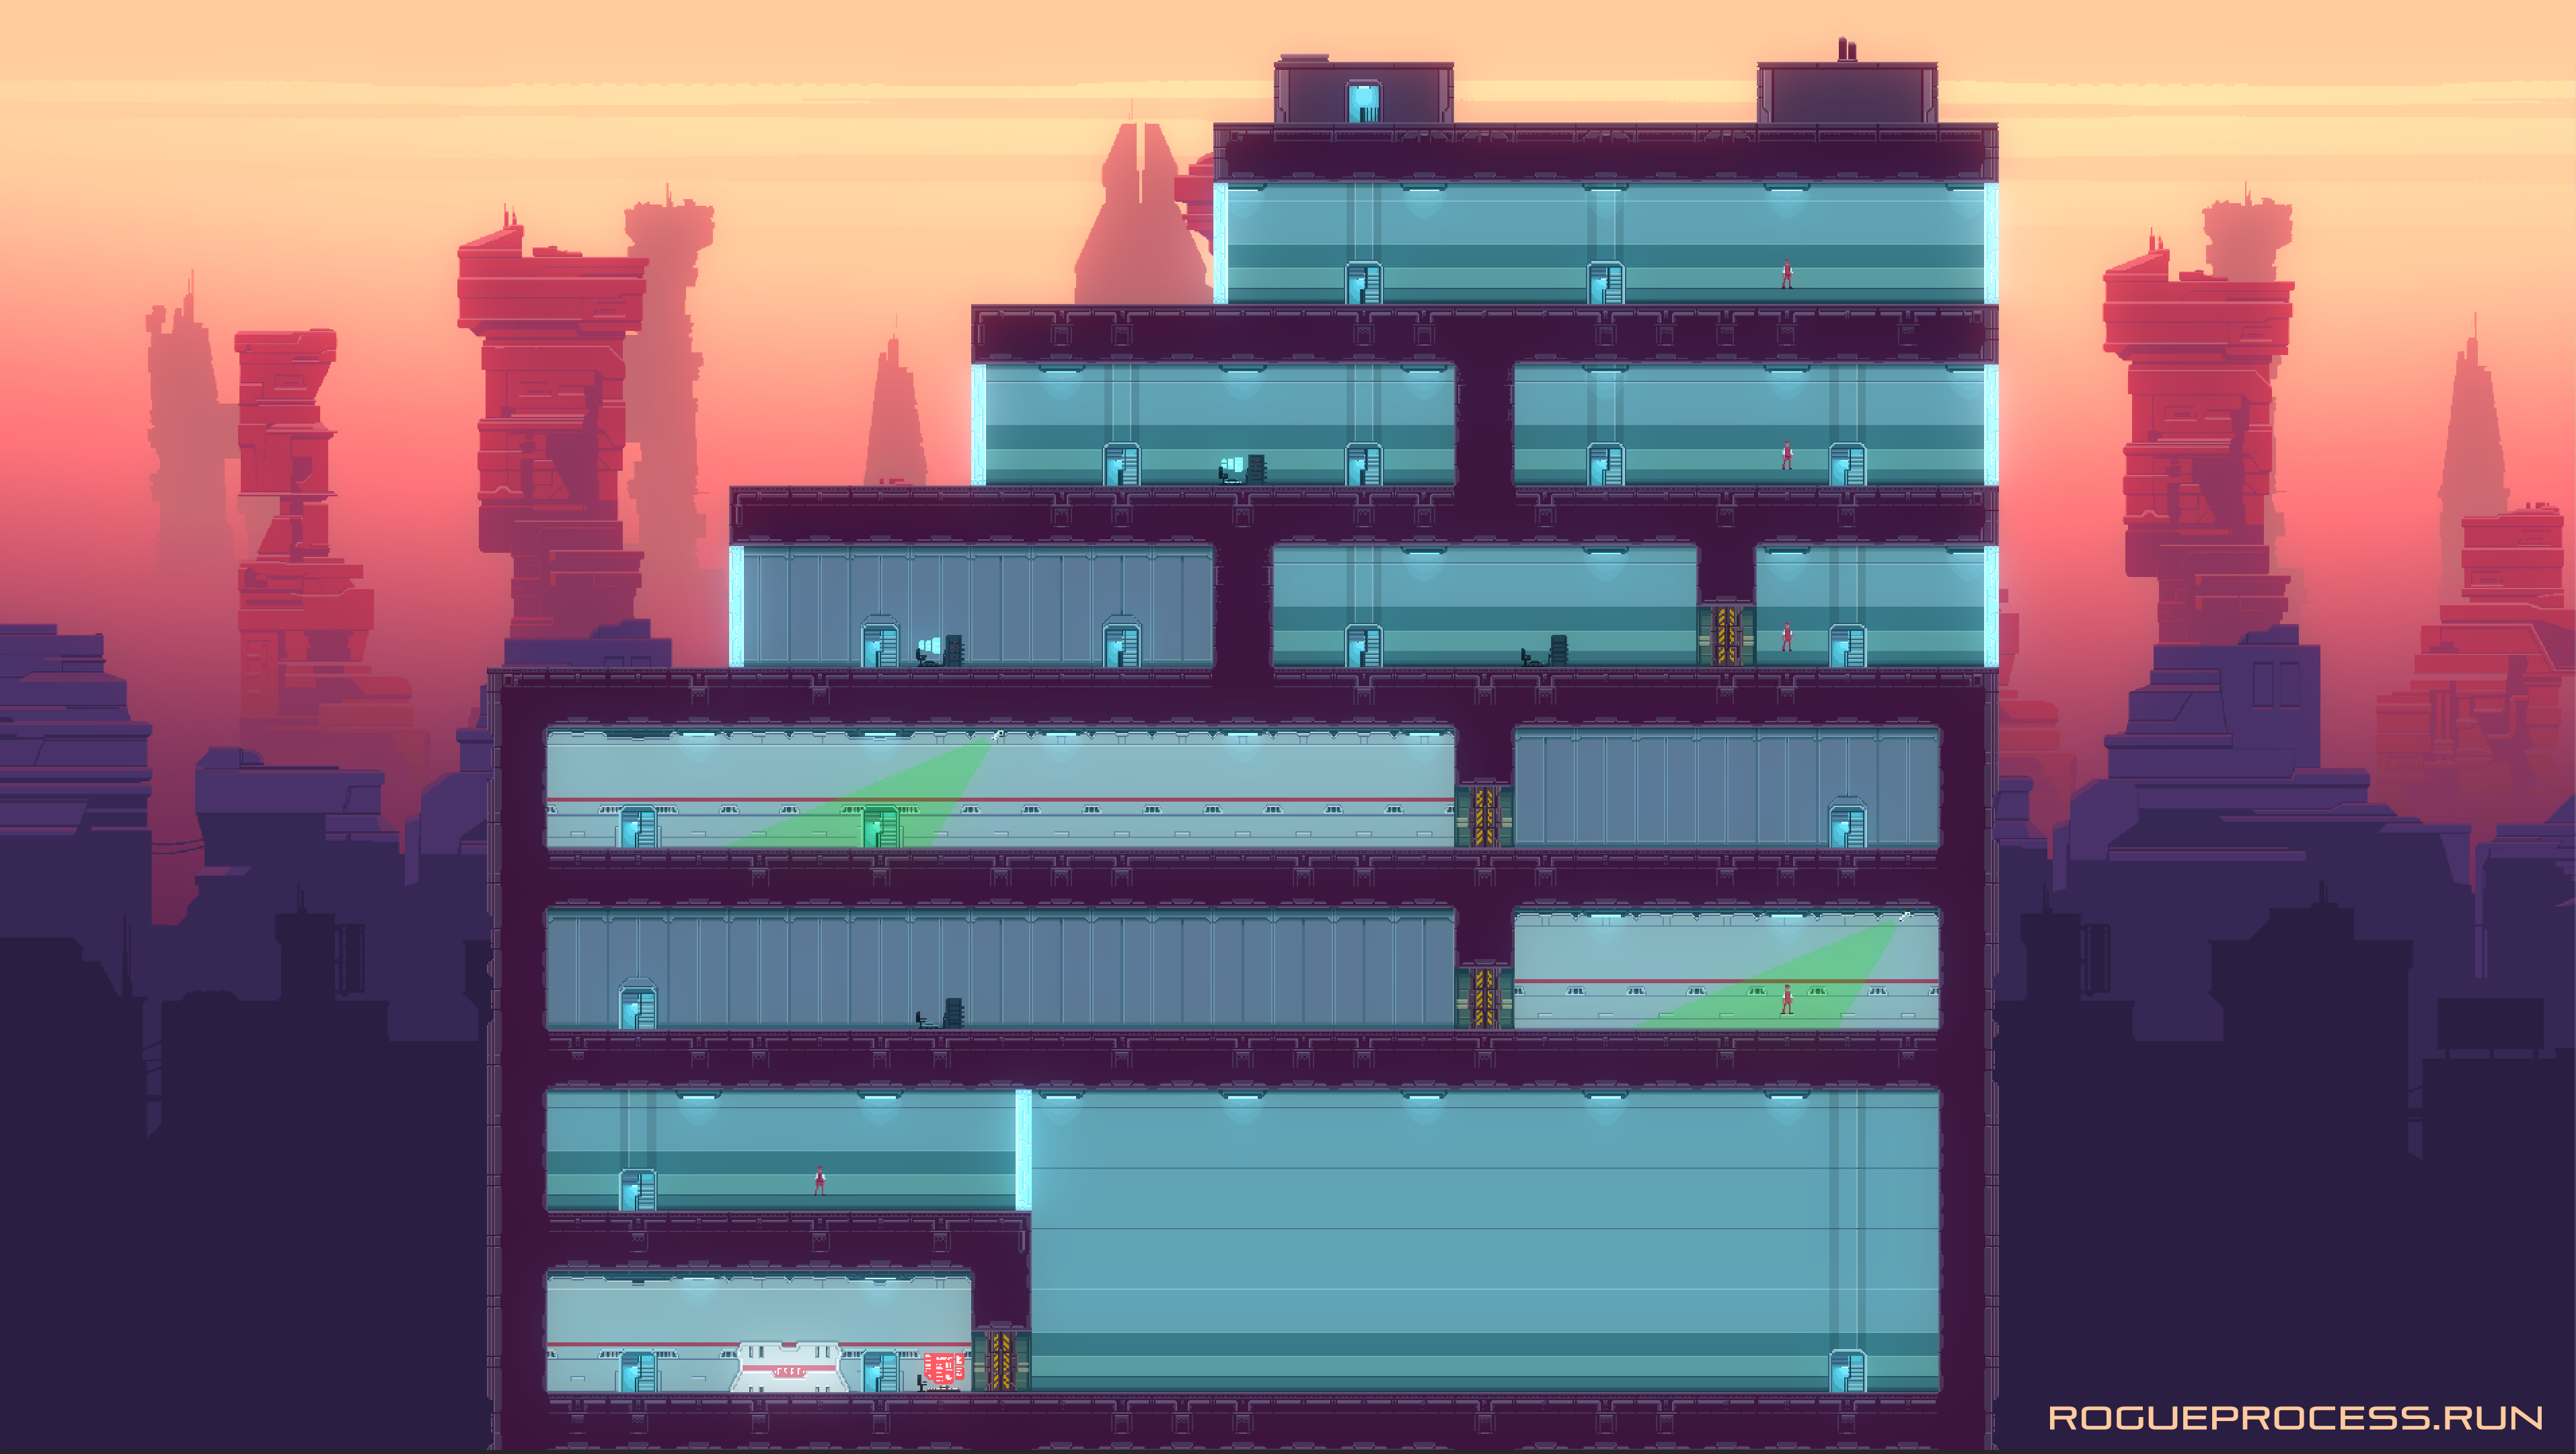
\includegraphics[width=\columnwidth]{images/rogue_process-screen}
  \caption{\textit{Rogue Process}: Example generated skyscraper for the player to infiltrate.}
  \label{fig:rp-setting}
\end{figure}


\textit{Rogue Process} (Figure~\ref{fig:rp-setting}) is an action hacking game about running through skyscrapers at high speeds and hacking their security networks in slow motion.
You play as a renegade hacker who makes their living stealing dark corporate secrets hidden away in the tops of skyscrapers.
It's being made by Michael Cook, with art and animation by Marsh Davies.
Music is currently courtesy of Strangelette.

Most of \textit{Rogue Process} takes place at the tops of skyscrapers, as the player breaks into various buildings in a city block to look for servers, prototypes and valuable data.
Skyscrapers are procedurally generated using logic-driven catalogue systems that define the relationship between elements of a building and allow natural structures to form from these rules.
They also allow for subtle emergent gameplay scenarios to emerge, because different room types offer different affordances to the player, allowing them to find alternate routes through a building, or solve problems in unexpected ways.
A chemical storage warehouse might be hacked to vent fuel into a room situated beneath it, which can then be set alight by a power surge sent to a cleaning robot, blowing an otherwise locked door off its hinges.

The worldbuilding of \textit{Rogue Process} is also heavily reliant on procedural systems.
Every building has a corporate owner, with a slogan, logo, specialism, name and relationship in the world generated through a combination of systems and approaches.
We're exploring the idea of `medium-permanence' PCG, where content is generated for an individual player, but it persists across multiple playthroughs, allowing the player to develop a longer-term relationship with the generated corporations instead of instantly discarding them.

Procedural generation extends throughout the game beyond these examples---the pedestrians in marketplaces, the ships in the background, the skylines they fly past.
We want the game to feel rich and varied, procedurally lavished with little details.

We're also using \textit{Rogue Process} as an opportunity to explore how procedural generation can be better supported in a developer workflow.
\textit{Danesh}, a tool for exploring generative spaces, was born out of prototype tools made for \textit{Rogue Process}, and we hope to continue to learn and expand on these ideas while working on the game and encountering new problems.

We're also hoping to just make a very fun game, and so we'd love you to come and play and tell us what you think.
There's a lot of interesting design issues to be solved within the game, especially reconciling precision typing with fast action, but we're enjoying exploring these problems and talking about them with players.
Visit us, have a go, and let us know what you think!

You can find out more about the game at \url{http://www.rogueprocess.run}, or on Twitter @rogue\_process


\section{Elsinore}

\begin{figure}[tbh]
  \centering
  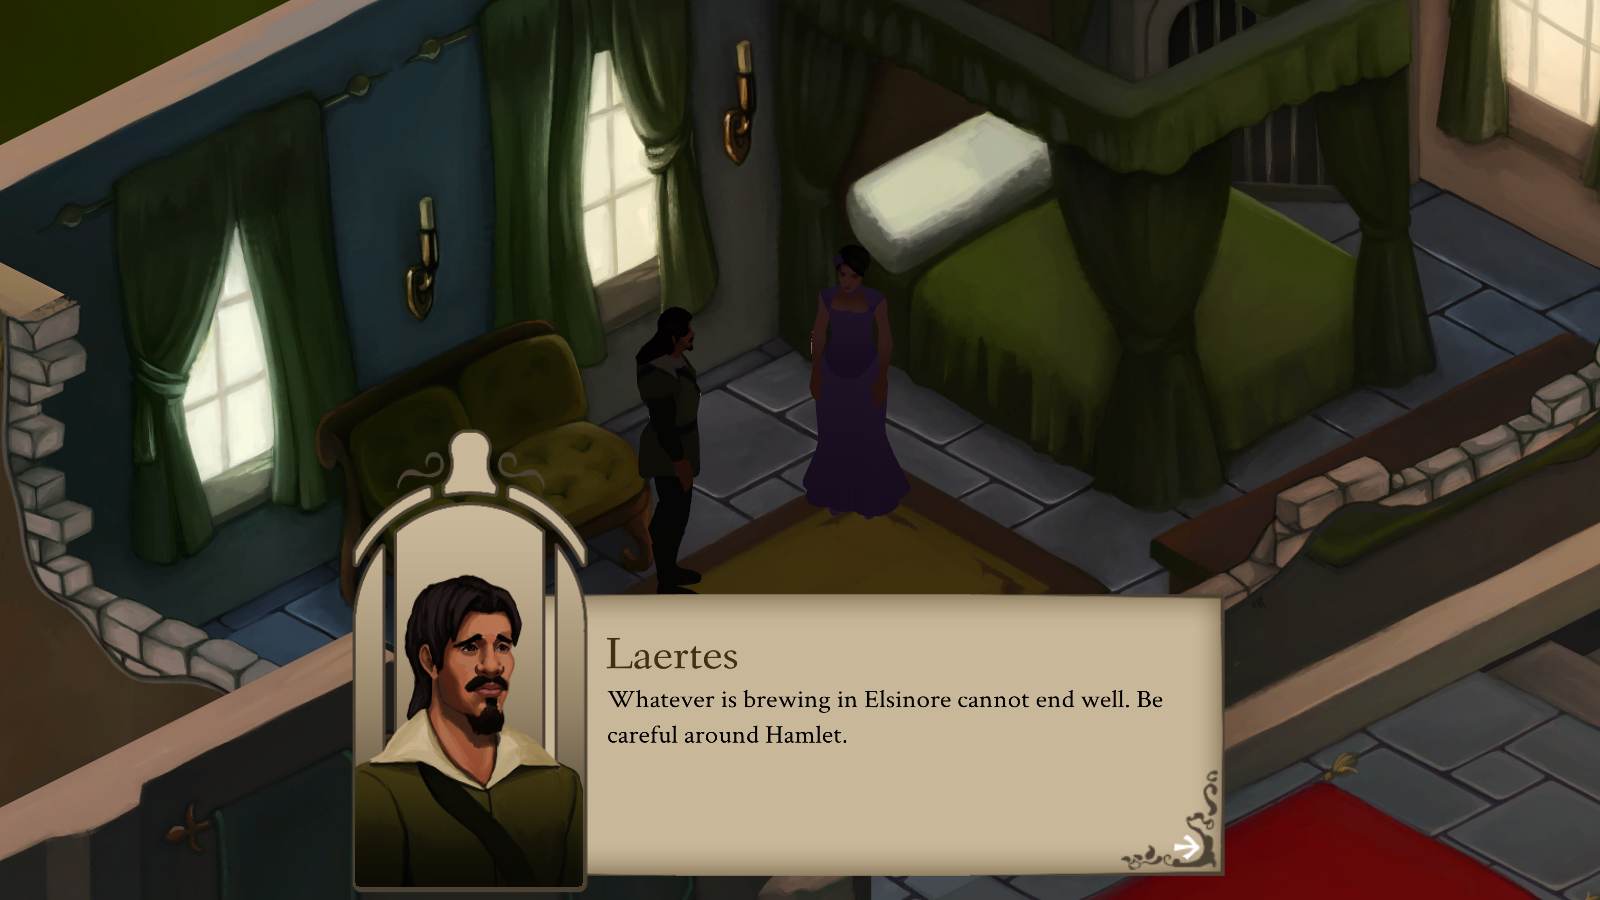
\includegraphics[width=\columnwidth]{images/elsinore-screen}
  \caption{\textit{Elsinore}: Example of the player witnessing an event in \textit{Elsinore}.}
  \label{fig:el-setting}
\end{figure}


\textit{Elsinore} is a time-looping adventure game set in the world of William Shakespeare's \textit{Hamlet}.
Players take on the role of Ophelia, navigating their way through Castle Elsinore and observing the events of the tragedy unfold in real-time.
Throughout the drama, Ophelia can acquire and present pieces of knowledge (called \textit{hearsay} in-game) to the other characters, influencing their beliefs and desires, changing the events that take place, and thus significantly affecting the final outcome.
Ophelia is trapped in a time loop, repeating the events of the play over and over.

\textit{Elsinore} combines hand-authored content and narrative simulation.
Individual scenes are hand-written but scheduled using a logic-based simulation.
The game state models the mental states of characters in a temporal predicate logic, and hand-authored events are preconditioned on these mental states.
These events occur in real time in a 3D environment; thus the simulation must schedule these events to avoid temporal conflicts with rooms and NPCs.
The player's primary tool, presenting \textit{hearsay}, changes these mental states, and accordingly, which events may occur.

The game's representation was chosen primarily to enable and assist the game experience.
One of the player's primary challenges is understanding how to manipulate the behavior of the NPCs to avoid a tragic outcome.
The NPC's mental states are exposed to the player.
This information aids the player in piecing together the mystery of the characters' behaviors and motivations, and how the player's actions affect the events and the endings.

The logic-based game state enables several AI techniques used to control the simulation, provide drama management, and support design tools.
For the simulation, the game uses propositional theorem proving to ensure important events are not suppressed by scheduling conflicts with minor events.
Events, by design, are non-interruptible once started.
Many major events can only happen at very specific times.
Therefore, if a minor event related to a sidequest were to be scheduled immediately before a major event and they both share a character or a room, the major event would be unable to occur.
However, in the cases where major events don't happen due to player action, we ideally want minor events to fill those gaps.
Therefore, our simulation schedules a minor event if, in addition to all typical preconditions, the game can prove that no conflicting major event could possibly happen within the duration of the minor event.
Given the logical preconditions, and postconditions, the duration, and the resources for every event, a hand-written propositional theorem prover can determine whether a minor event should be allowed to happen.

Our game also uses this logical model for minor drama management.
While exploring the castle, the player may engage in idle conversations with other NPCs.
These conversations cannot change the logical state, though, like the rest of game's dialogue, it is determined by logical state.
We can use this idle conversation to guide the player.
NPCs discuss relevant and topical information with the player, such as reactions to character deaths.
They also often inform the player about important scenes that the player did not witness or remind them of upcoming important events.

\begin{figure}[tbh]
  \centering
  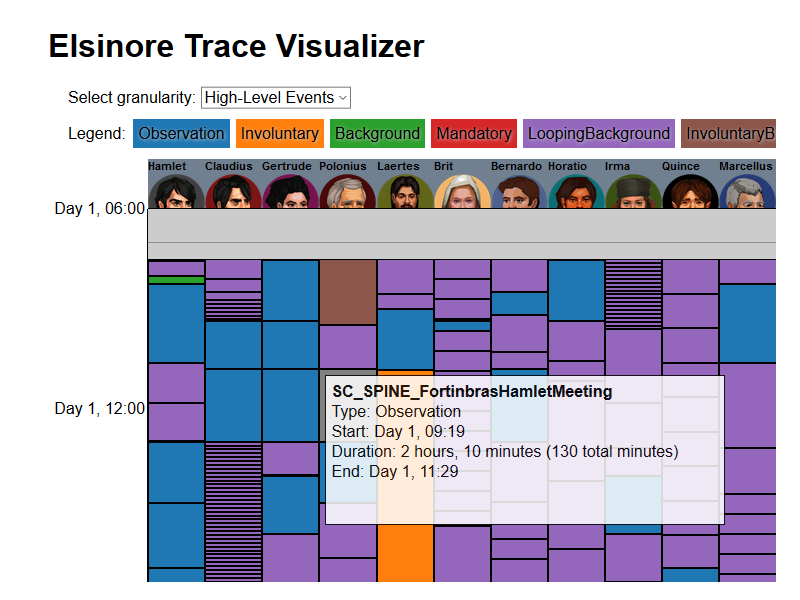
\includegraphics[width=\columnwidth]{images/elsinore-tool}
  \caption{\textit{Elsinore}: Sample event trace from the \textit{Elsinore} visualization tool. Colored boxes represent different kinds of events, with attending characters and scheduled time along the axes.}
  \label{fig:el-tool}
\end{figure}

Finally, we are using AI to support our design workflow.
Currently, our design tools are capable of visualizing game traces and performing static analysis of game scripts.
We are in the process of developing solver-powered design tools for automatic QA and computational critics.
Exploiting the discrete, logical representation and event simulation, we are using off-the-shelf tools such as SMT solvers to reason about an abstracted version of the game.
This allows us to answer game-design-relevant questions such as event reachability, and will hopefully support more sophisticated queries as development progresses.

Information about the game can be found at \url{https://elsinore-game.com/}.



\section{Conceptually Blended Levels in a Unity Engine}

\begin{figure}[tbh]
  \centering
  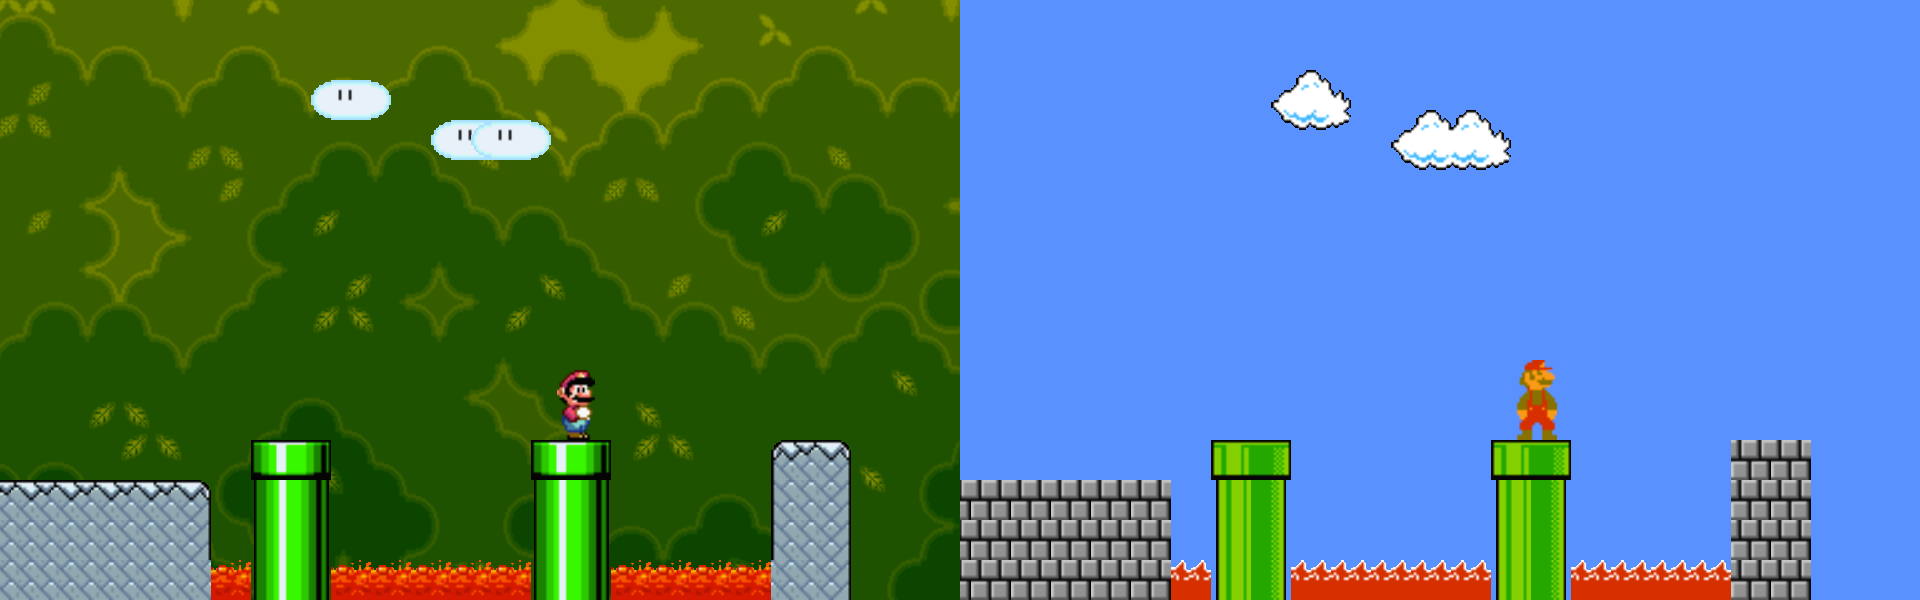
\includegraphics[width=\columnwidth]{images/conceptual_blend-screen}
  \caption{\textit{Conceptually Blended Levels}: Example level and blend.}
  \label{fig:cb-placeholder}
\end{figure}

We present a system that generates playable output in the style of \textit{Super Mario Bros.} using an unsupervised approach for concept blending models of level design.
The concept blending requires a goal and a set of probabilistic models composed of probabilistic, spatial relationships between level components.
The output of this approach is a blended probabilistic model that can be used for generation and evaluation.
The playable experience is a set of generated output from these blended models, along with their relative evaluations.

We first introduced these probabilistc models in ``Towards Game Level Generation from Gameplay Videos'' \cite{guzdial2015:video-level-gen}.
They are derived via a hierarchical, unsupervised clustering method that learns styles of levels and of level components from gameplay video.
We have since extended these probabilistic models with concept blending \cite{guzdial2016:mario-blend}.
Concept blending describes a process of merging disparate concepts into a blended whole, generally via mapping components of two concepts onto one another in order to reach some ``target'' concept.
We make use of analogical reasoning to map relationships from one probabilistic model onto another in order to reach a specified target.
The levels present in this demo represent the output of conceptually blended models with a variety of targets, including levels from the game \textit{Super Mario Bros.: The Lost Levels} and more abstract specifications such as ``underwater castle.''

We encode the levels within a new, open-source \textit{Super Mario Bros.} Unity engine\footnote{\url{http://guzdial.com/unitySMB}}.
The engine allows us to encode levels that could not previously be played, including underwater levels, castle levels, and our own conceptually blended output.
In addition the engine allows drag-and-drop changes to levels, multiple players, and multiple ``skins'' for each level (including \textit{Super Mario Bros.} and \textit{Super Mario World}).
We hope that this engine will benefit the broader Game AI community.

To the best of our knowledge, this represents the first time that conceptually blended video game levels have been made playable at a public event.
Despite the popularity of automatic level generation as a research topic, it is fairly unusual for the output of generators to be made publicly playable.
We hope that this demonstration inspires more level generation researchers to make output that is publicly playable.


\section{Bad News}
\subsection{Summary}
\textit{Bad News} is a novel playable experience that combines procedural generation, deep simulation, and live performance. Players explore procedurally generated American small towns inhabited by detailed characters with simulated backstories. Whenever the player encounters a resident, an improvisational actor reveals himself to perform the character live, adhering to his or her generated personality, life history, and subjective beliefs. With \textit{Bad News}, we strive to showcase the humor, drama, and tragedy of everyday life.


\subsection{How To Play}

It is the summer of 1979, and an unidentified resident of a small American town has died alone at home. The county mortician is responsible for identifying the body and notifying the next of kin, but a matter in a different part of the county demands his presence. Being occupied in this way, the mortician is forced to delegate this important task to his newly appointed assistant, the player. To carry out the task, the player must navigate the town and converse with its residents in order to obtain three crucial pieces of information, each of which can only be discovered by knowing the preceding piece: the identity of the deceased, given only the person's physical appearance and home; the identity of the next of kin, given the identity of the deceased and an explicit notion of a next of kin (that we provide); and the current location of the next of kin, given his or her identity and any other relevant information that the player has gathered. Finally, upon locating the next of kin, the player must notify him or her of the death. Throughout, she should remain discreet, so as to respect the privacy of the family.

The player sits on one side of a constructed model theatre (shown in Figure~\ref{fig:bn-model_theatre}), with a tablet computer, a notebook, and a pen. A live actor sits across from the player, hidden by the theatre's adjustable curtain; behind a permanent lower curtain, a hidden screen displays a special actor interface and a discreet microphone captures sound. Out of sight, a \textit{wizard} listens to the audio feed. Gameplay always begins at the death scene, where the actor reveals himself to play the mortician, who explains what has happened and what the player must now do. This happens diegetically and occurs as embodied face-to-face conversation; the purpose of this scene is to subtly tutorialize and to gently ease the player into both the diegesis and the live-action role-playing that the experience requires. Crucially, the mortician and the player collaborate to construct a believable backstory that the player can rely on when talking with residents in the town---after all, it would not be discreet to openly parade as the mortician's assistant. From here, the mortician disappears by deploying the curtain, and the player is left with the tablet computer (see Figure~\ref{fig:bn-player_interface}), which displays a player interface that initially describes her current location (including the body).

\begin{figure}[t]
  \centering
  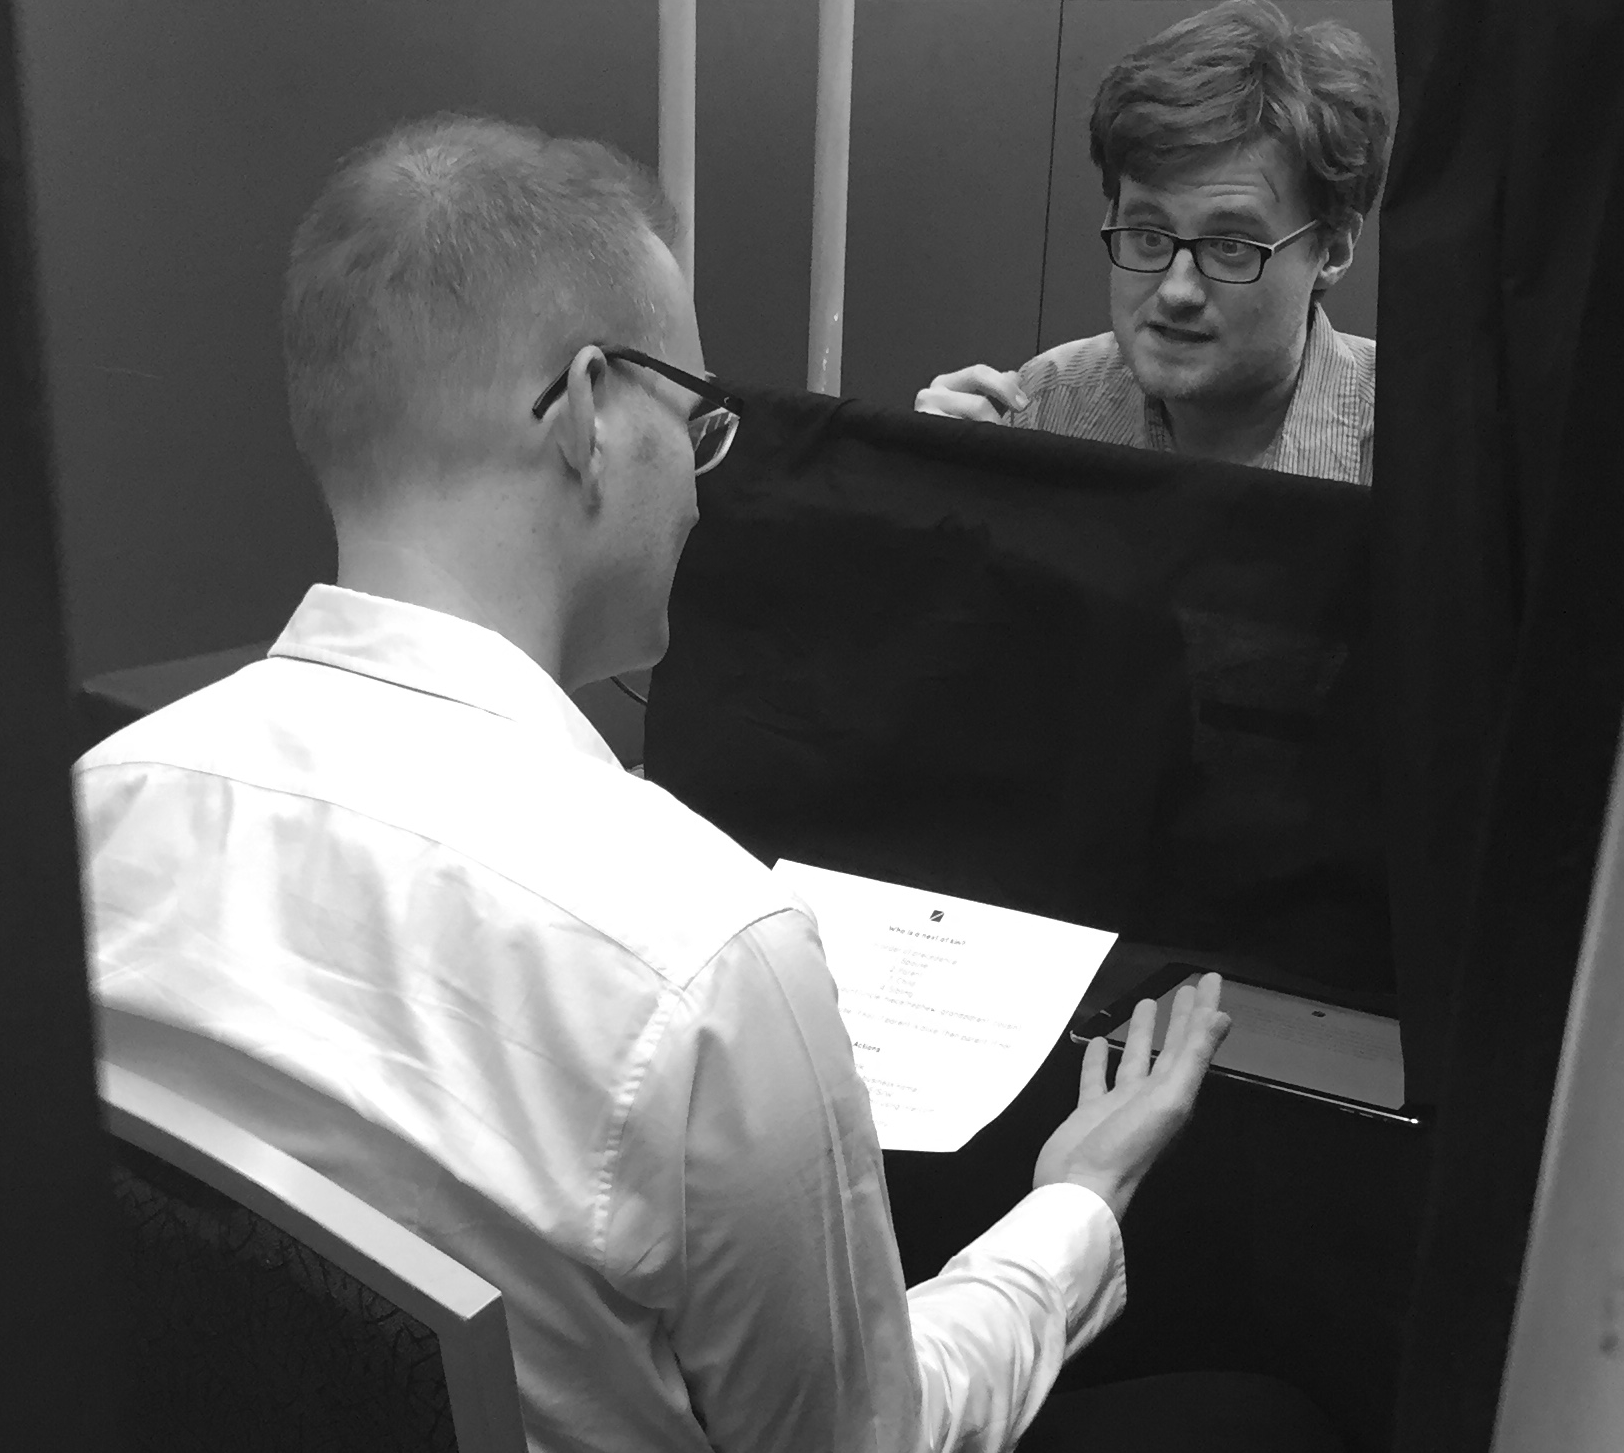
\includegraphics[width=0.8\columnwidth]{images/bad_news-player_and_actor}
%  \vspace{-2.0em}
  \caption{\textit{Bad News}: A player, left, engages in embodied conversation with the actor, who improvisationally performs as a resident of the town.}
  \label{fig:bn-player_and_actor}
\end{figure}

From here, the player proceeds by speaking commands aloud; the wizard executes these throughout the experience by live-coding modifications to the simulation in real time. Permissible commands include moving about the town (in a direction, or to an address), viewing a residential or business directory, approaching a character to engage in conversation, and more. As the player moves about the town, her interface updates to describe her current location. When a player approaches a town resident, the hidden actor interface updates to display details about that character's personality, life history, and subjective beliefs. After spending a few moments preparing for the role, the actor pulls back the curtain to play that character live. As the subject of conversation shifts between residents of the town, the wizard crucially updates the actor interface to display the character's beliefs about that particular resident. Meanwhile, the wizard queries the simulation for narrative intrigue (again by live-coding), which he can deliver to the actor directly through a live chat session (\textit{e.g.}, ``you went to high school with the subject''). Gameplay ends once the player notifies the next of kin of the death. A typical session lasts roughly 45 minutes, though the wizard and actor can coordinate in real time to control this. For more details, see our longer paper \cite{samuel2016bad}.


\subsection{Why To Play}


\begin{figure}[t]
  \centering
  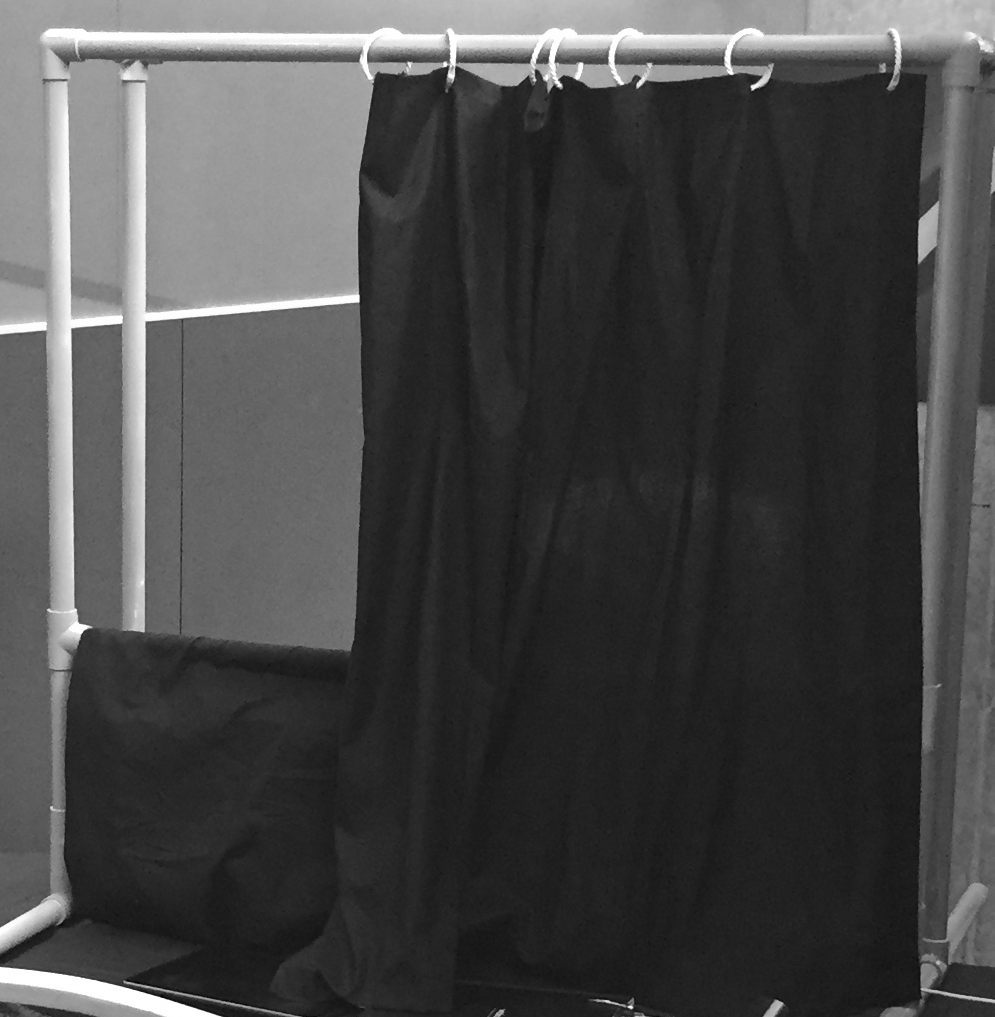
\includegraphics[width=0.64\columnwidth]{images/bad_news-the_puppet_theatre}
  \caption{\textit{Bad News}: A constructed model theatre separates the player and our live actor.}
  \label{fig:bn-model_theatre}
\end{figure}

\textit{Bad News} is appealing as a novel, AI-driven, and tender experience. While \textit{mixed reality} is a growing and fairly active area \cite{ohta2014mixed}, there are surprisingly few media works that specifically combine computation and live improvisation. In fact, we are aware of only two other examples of this---\textit{Coffee: A Misunderstanding} \cite{squinkifer2014coffee} and \textit{S\'{e}ance} \cite{seance}---though interest is growing \cite{martens2016towards}. Incidentally, \textit{S\'{e}ance} features our same actor, Ben Samuel, who appears to be the world's expert in improvisational acting under computational constraints; watching him perform in myriad roles is a core appeal of the experience. Beyond its novelty, this work is deeply AI-driven. Each \textit{Bad News} town is procedurally generated using the \textit{Talk of the Town} AI framework \cite{ryan2015toward}. Specifically, towns are simulated for 140 years of diegetic time, yielding hundreds of residents who are socially embedded and who harbor subjective beliefs about the town (which may be wrong for multiple interesting reasons). This provides an abundance of narrative material and dramatic intrigue (\textit{e.g.}, family feuds, love triangles, struggling businesses) that exceeds the capacities of a 45-minute playthrough and that could not have tractably been hand-authored. Several players have reported feeling like they were \textit{transported} to the generated towns that they visited \cite{green2004understanding}. Finally, \textit{Bad News} is a tender experience. As a game about death notification, it compels the player to be sincere and tactful---many have commented on the emotional intensity of their notification scenes. Set in run-of-the-mill American small towns, we strive in each playthrough, through acting and wizardry, to showcase the humor, drama, and tragedy of everyday life.

\subsection{Where To Play}

\begin{figure}[t]
  \centering
  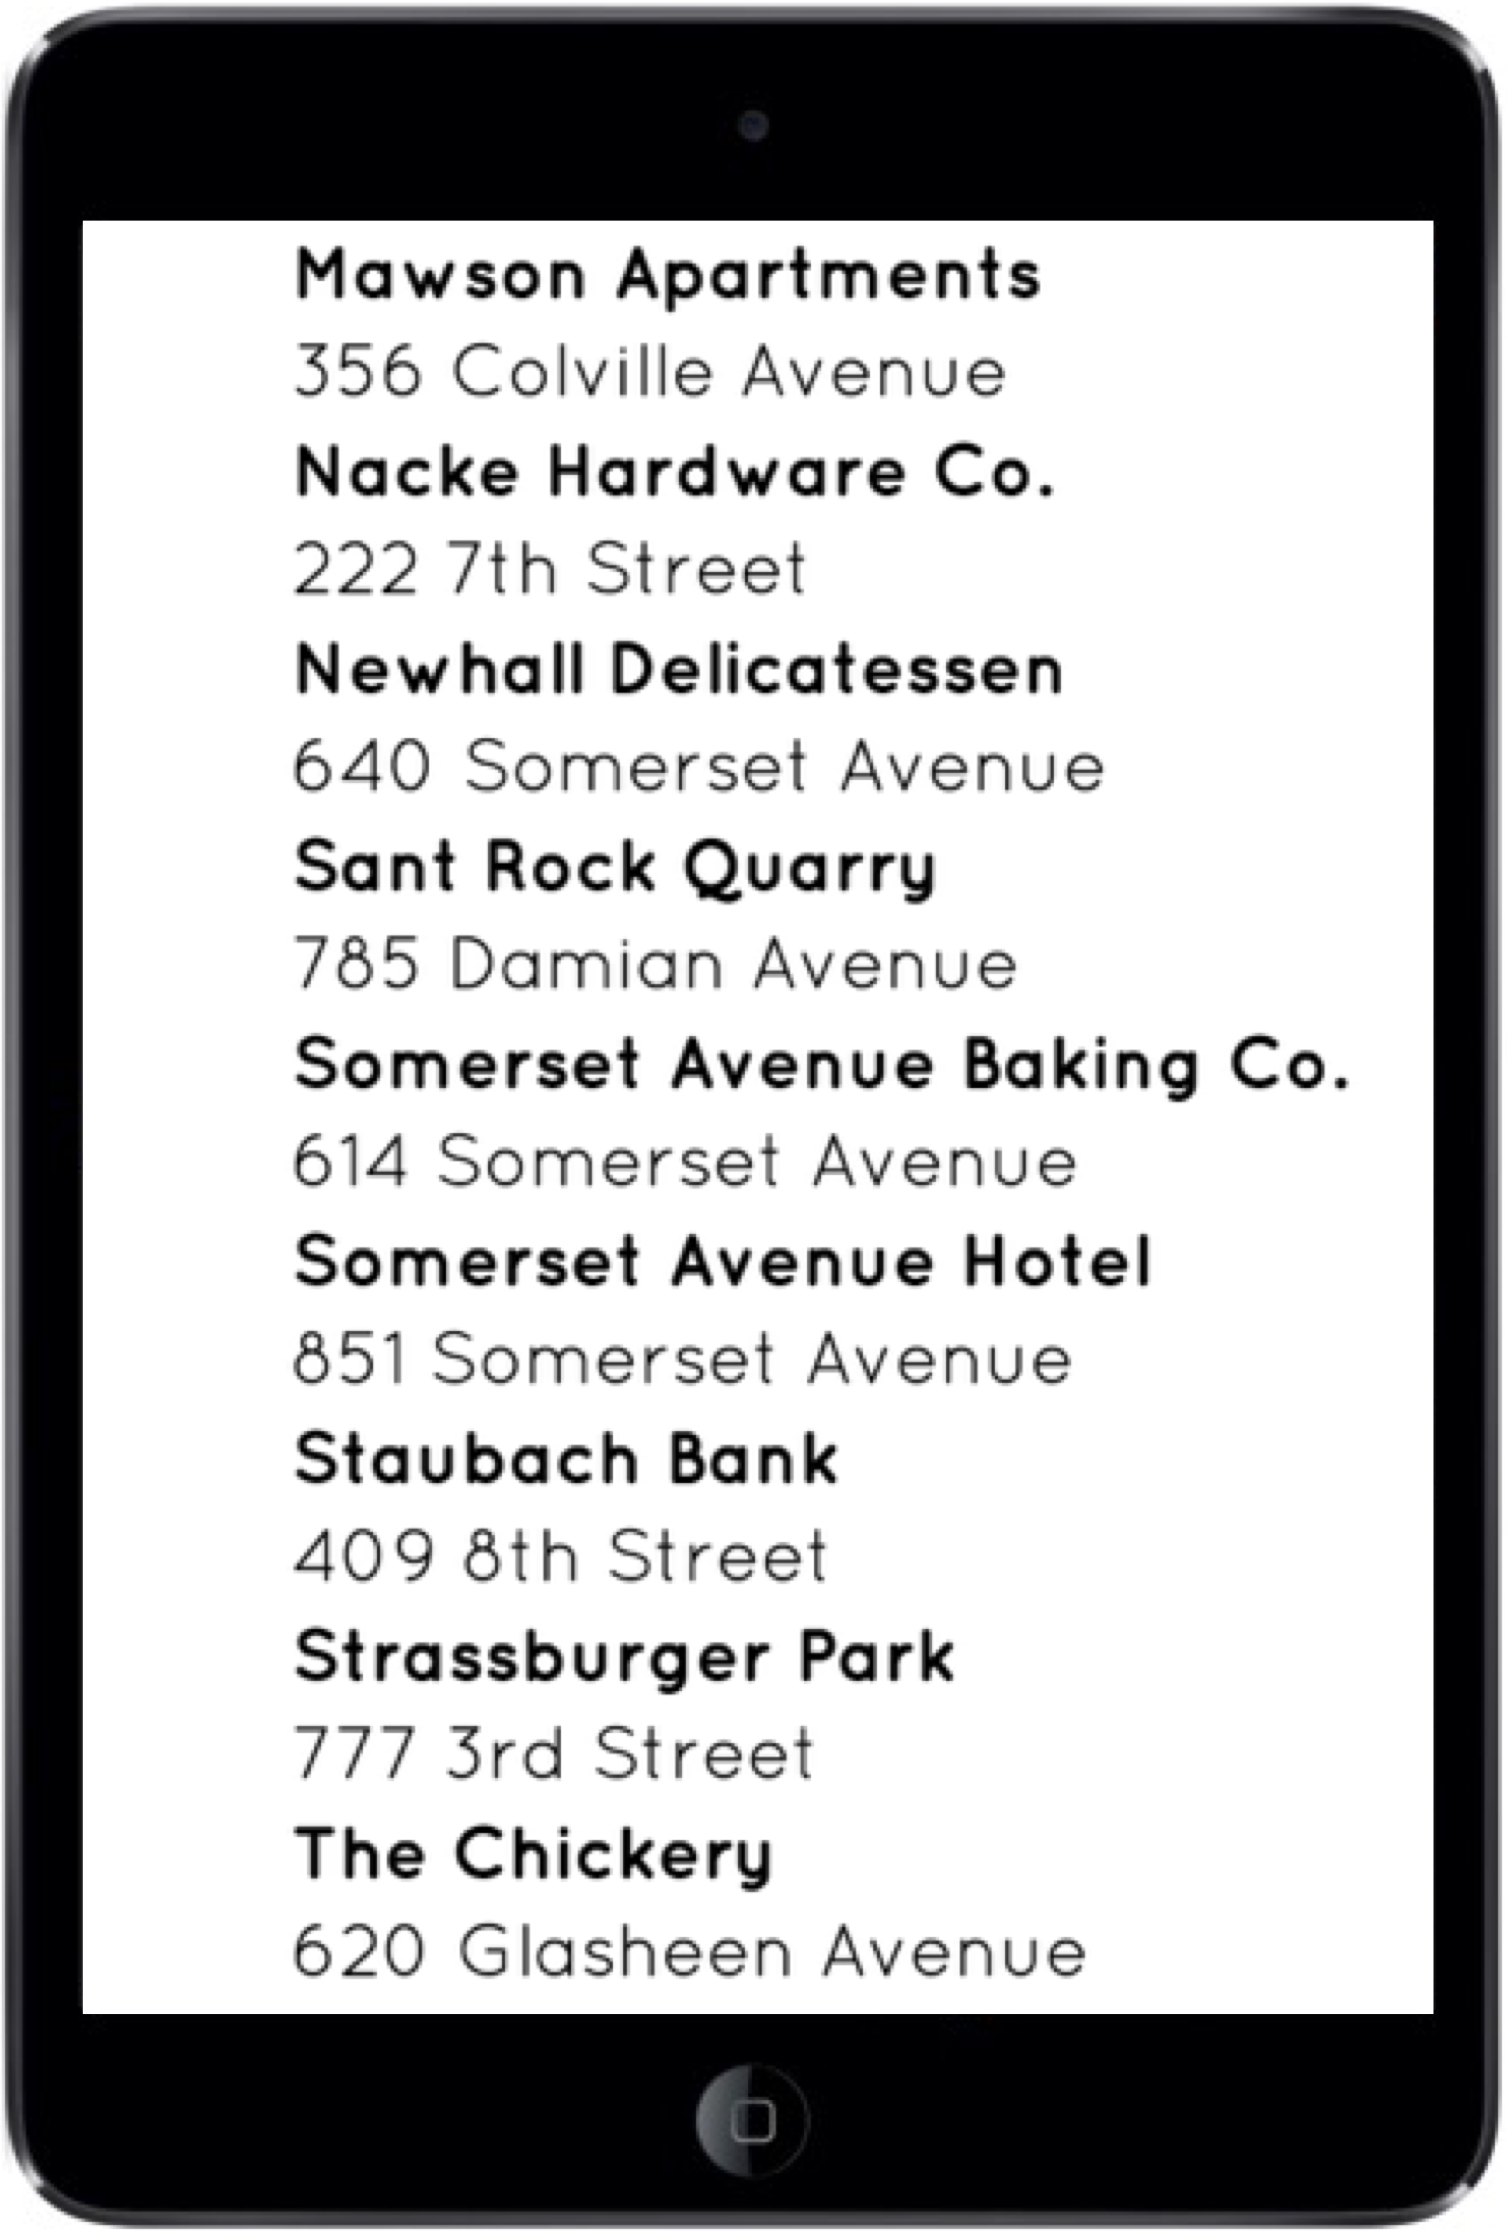
\includegraphics[width=0.42\columnwidth]{images/bad_news-player_interface}
  \caption{\textit{Bad News}: Excerpt from a business directory for a procedurally generated town, as displayed on the player interface.}
  \label{fig:bn-player_interface}
\end{figure}

Because the actor and wizard must both be present, \textit{Bad News} can only be played in person at scheduled performances. Though we have accommodated private requests, it is primarily intended as an exhibition piece. An early test incarnation was conducted at the 2015 Experimental AI in Games workshop in Santa Cruz \cite{ryan2015bad}, and more recently our refined, longer version was performed at the ACM Conference on Human Factors in Computing Systems (CHI) in San Jose \cite{ryan2016bad} and at Gamenest in San Francisco. The middle performance was part of the Innovative Game Design track of the CHI Student Game Competition, which \textit{Bad News} won.



%The following commands are available for your use in citing references:
%\begin{quote}
%\begin{small}
%\textbackslash cite: Cites the given reference(s) with a full citation. This appears as ``(Author Year)'' for one reference, or ``(Author Year; Author Year)'' for multiple references.\\
%\textbackslash shortcite: Cites the given reference(s) with just the year. This appears as ``(Year)'' for one reference, or ``(Year; Year)'' for multiple references.\\
%\textbackslash citeauthor: Cites the given reference(s) with just the author name(s) and no parentheses.\\
%\textbackslash citeyear: Cites the given reference(s) with just the date(s) and no parentheses.
%\end{small}
%\end{quote}




\bibliography{lib}
\bibliographystyle{aaai}

\end{document}
